% =============================================================================
% Part II, Chapter 4: The Experimental Infrastructure
% =============================================================================
\chapter{The Experimental Infrastructure}\label{ch:infrastructure}

Empirical findings in LLM evaluation are only as trustworthy as the software, inference server, quantization pipeline, parser, and audit trail that produced them. Across CausalFade's twenty-nine-day history, infrastructure bugs and subtle execution defaults repeatedly masqueraded as cognitive discoveries---from Markdown code-fence mismatches in Cohort~001 to noncausal length-cap truncations in Cohort~024 and option-order coupling in Cohort~026. Equally important, every time such an artifact was uncovered, the researchers hardened the engineering stack rather than patching results by hand. This chapter documents the technical architecture of CausalFade and traces how its reproducibility safeguards evolved across four infrastructure generations (Figure~\ref{fig:infra_arch}).

\begin{figure}[htbp]
  \centering
  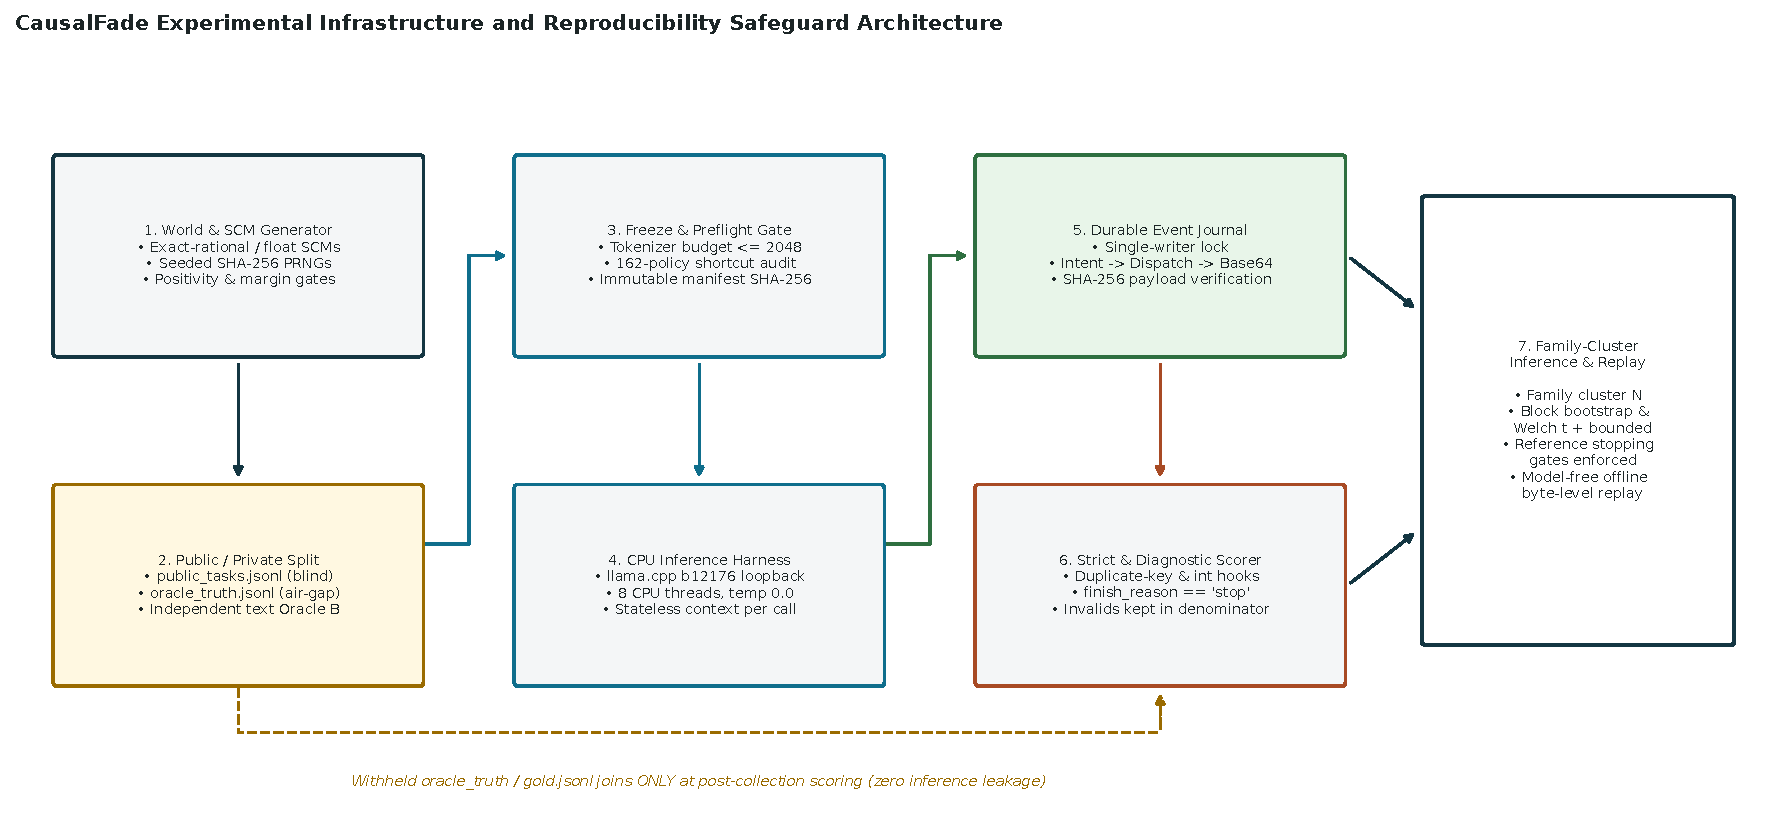
\includegraphics[width=\textwidth]{figures/fig07_infrastructure_architecture.pdf}
  \caption{End-to-end technical architecture of Project CausalFade, illustrating the strict air-gap between public prompt manifests and evaluator-only oracle truth, deterministic local \texttt{llama-server} execution, raw response journaling, strict vs.\ normalized parser layers, and family-clustered statistical scoring.}
  \label{fig:infra_arch}
\end{figure}

% =============================================================================
\section{Repository Organization and Four-Generation Evolution}

At snapshot commit \nolinkurl{b7371530caa62d6e43a8e83ef6db361f6640f63a}, the repository is organized into six functional layers:
\begin{enumerate}
  \item \textbf{Core Python Package (\texttt{causalfade/}):} Built during the initial validation phase (commits \texttt{6ab18d2}--\texttt{caf5b1d}), containing \texttt{scm.py} (binary backdoor SCM construction), \texttt{generate.py} (world family sampling and JSONL serialization), \texttt{cab\_tree.py} (multinomial processing tree EM solver and bootstrap deviance tests), \texttt{evaluate.py} (JSON response parsing and metric aggregation), and \texttt{runner.py} (local HTTP client against \texttt{llama-server}).
  \item \textbf{Operational Harnesses and Utilities (\texttt{tools/}):} Cohort-specific dataset builders, model preflight verifiers, RAM safety guards, deterministic calculator sandboxes (Cohort~028), and standalone audit scripts.
  \item \textbf{Pre-LLM Synthetic Validation (\texttt{results/design\_validation/}):} Frozen synthetic parameter-recovery artifacts ($3{,}600$ EM fits), logistic observational equivalence checks, and the initial $24$-family ($192$-prompt) testbed.
  \item \textbf{Experimental Cohort Archive (\texttt{experiments/cohort\_001/} through \texttt{cohort\_029/}):} Thirty self-contained cohort directories (including \texttt{cohort\_025\_1}) preserving input manifests, schedules, server logs, raw JSONL model responses, scored JSON summaries, and contemporaneous Markdown reports.
  \item \textbf{Governance and Audit Documentation (\texttt{EXPERIMENTS.md}, \texttt{DECISIONS.md}, \texttt{docs/}):} Chronological ledgers recording pre-execution contracts, hardware reuse manifests (\texttt{docs/SSD\_ASSET\_REUSE.md}), data contracts (\texttt{docs/DATA\_CONTRACT.md}), statistical analysis plans (\texttt{docs/STATISTICAL\_ANALYSIS\_PLAN.md}), and retrospective readiness audits.
  \item \textbf{Final Manuscript Package (\texttt{manuscript/}):} Self-contained publication source (\texttt{article.tex}, \texttt{supplement.tex}, \texttt{history.tex}), byte-level reconstruction scripts (\texttt{manuscript/scripts/extract.py}, \texttt{figures.py}), and claim-audit ledgers (\texttt{manuscript/audit/claim-ledger.csv}).
\end{enumerate}

Crucially, the experimental runner evolved through four distinct generations:
\begin{itemize}
  \item \textbf{Gen~1 (Cohorts~001--011):} Core \texttt{causalfade} runner over single-table backdoor JSON prompts (\texttt{max\_tokens=160}, temperature $0.0$), expanded in Cohort~002 with a dual parser layer separating strict bare-JSON parsing from code-fence-stripped diagnostic parsing.
  \item \textbf{Gen~2 (Cohorts~012--023):} Two-study evidence-selection pipeline introducing bare single-key JSON contracts (\texttt{\{"activate": 1\}}, \texttt{\{"choice": "M"\}}, \texttt{\{"decision": "activate"\}}), prompt-order counterbalancing, and component sub-skill probes.
  \item \textbf{Gen~3 (Cohorts~024--028):} Cross-lineage multi-precision matrix runner ($21$ arms in Cohort~024), bare-token graph-switch evaluators (Cohorts~026--027), and Cohort~028's two-stage structured JSON + allowlisted Python deterministic calculator (\texttt{System C}).
  \item \textbf{Gen~4 (Cohort~029, \texttt{CF-TP1}):} Pre-registered cryptographic freeze architecture (\texttt{experiments/cohort\_029/freeze/}) featuring exact-rational \texttt{fractions.Fraction} SCM synthesis, $162$-policy pre-run shortcut auditing, blinded human/scripted fixture review, and an append-only base64-encoded HTTP response journal (\texttt{events.jsonl}) cryptographically bound to the frozen manifest SHA-256 (\texttt{5252f69d...}).
\end{itemize}

% =============================================================================
\section{Hardware Environments and Local Inference Stack}

All $48{,}170$ persisted LLM responses in CausalFade were executed locally on CPU/UMA consumer workstation hardware running Linux/WSL2 and Windows host storage without external cloud APIs, ensuring bit-for-bit control over model weights, quantization kernels, and decoding settings (\texttt{docs/SSD\_ASSET\_REUSE.md} and run \texttt{metadata.json} logs):
\begin{itemize}
  \item \textbf{Host Memory \& Safety Guardrails:} $32\;\text{GiB}$ system RAM ceiling. In Cohort~017, running \texttt{Qwen2.5-14B} required substituting \texttt{Q8\_0} ($14.6\;\text{GiB}$) for \texttt{F16} ($\approx 29.5\;\text{GiB}$), and in Cohort~027 pre-run RAM safety checks (\texttt{experiments/cohort\_027/README.md}) formally excluded \texttt{Qwen2.5-14B F16} before execution to prevent swap thrashing or out-of-memory termination.
  \item \textbf{Inference Engine:} \texttt{llama.cpp} HTTP server (\texttt{llama-server}, build \texttt{b12176-8820b088d} in early cohorts and consistent OpenAI-compatible \texttt{/v1/chat/completions} endpoints throughout), queried sequentially (\texttt{parallel=1}) with $8$ CPU threads (\texttt{threads=8}), deterministic greedy decoding (\texttt{temperature=0.0}), explicit integer RNG seeds (e.g., \texttt{20261110} in Cohort~001; \texttt{20261125} in Cohort~029), and zero KV-cache prompt cross-contamination across independent requests.
\end{itemize}

% =============================================================================
\section{Model Lineages and GGUF Quantization Provenance}

Across its asset inventory and active experiments, CausalFade prepared or evaluated five parameter scales across three open-weight instruction-tuned transformer lineages (Figure~\ref{fig:model_matrix}; full cryptographic details in Appendix~C, Table~\ref{tab:model_quant_inventory}):
\begin{enumerate}
  \item \textbf{Qwen2.5-Instruct Family:} \texttt{0.5B} and \texttt{1.5B} (prepared on local SSD in \texttt{F16, Q8\_0, Q4\_K\_M, Q2\_K, Q1\_0} via \texttt{llama-quantize b12176} without an importance matrix, documented in \texttt{docs/SSD\_ASSET\_REUSE.md}, but never queried in Cohorts~001--029); \texttt{3B} (workhorse of Cohorts~001--011 and 027); \texttt{7B} (primary model of Cohorts~012--029, including all $7$ formats in Cohort~024 and \texttt{Q4\_K\_M} in Cohort~029); and \texttt{14B} (\texttt{Q8\_0} and \texttt{Q4\_K\_M} in Cohort~017).
  \item \textbf{Mistral-7B-Instruct-v0.3:} Evaluated in Cohorts~022, 023, 024 (all $7$ GGUF formats: \texttt{F16, Q8\_0, Q6\_K, Q5\_K\_M, Q4\_K\_M, Q3\_K\_M, Q2\_K}), and 027 (\texttt{F16}).
  \item \textbf{Meta-Llama-3.1-8B-Instruct:} Evaluated in Cohorts~024 (all $7$ GGUF formats), 026 (\texttt{F16}), 027 (\texttt{F16}), and 028 (\texttt{F16}).
\end{enumerate}

\begin{figure}[htbp]
  \centering
  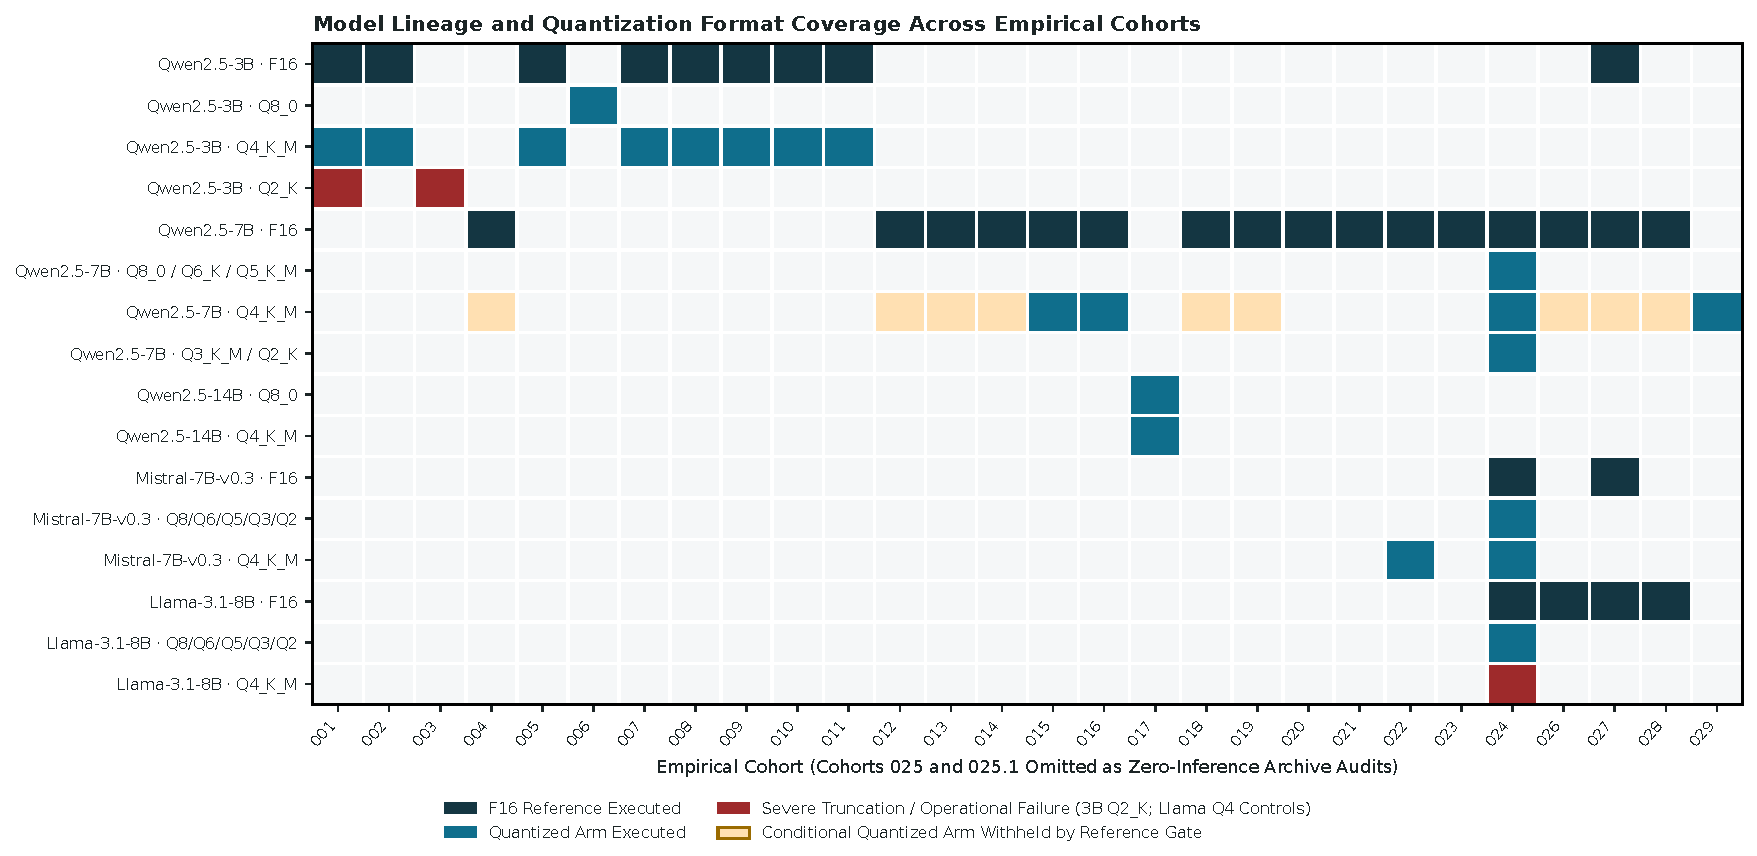
\includegraphics[width=\textwidth]{figures/fig06_model_cohort_matrix.pdf}
  \caption{Model-by-cohort deployment matrix across all 30 empirical cohorts, illustrating the progression from \texttt{Qwen2.5-3B} pilots (001--011) to \texttt{Qwen2.5-7B/14B} two-study cohorts (012--021), cross-lineage \texttt{Mistral-7B} and \texttt{Llama-3.1-8B} matrices (022--028), and the confirmatory \texttt{Qwen2.5-7B Q4\_K\_M} run (029).}
  \label{fig:model_matrix}
\end{figure}

Every run directory recorded the exact GGUF file path and, in manifest-hardened cohorts, the full 64-character SHA-256 digest of the model weights (for example, \texttt{qwen2.5-3b-instruct-f16.gguf} = \texttt{7861b687...} in Cohort~001, and \texttt{Qwen2.5-7B-Instruct-Q4\_K\_M.gguf} verified in Cohort~029's frozen manifest). In Cohort~001, \texttt{tokenizer\_metadata\_audit.json} explicitly verified that GGUF header chat templates, BOS/EOS tokens, and vocabulary tables were identical across \texttt{F16}, \texttt{Q4\_K\_M}, and \texttt{Q2\_K}, ruling out tokenizer corruption as an explanation for low-bit failures.

% =============================================================================
\section{Blind Data Contracts, Randomization, Parsing, and Logging}

Four architectural safeguards prevented subtle evaluation leakage throughout CausalFade:
\begin{enumerate}
  \item \textbf{Public-Oracle Air Gap (\texttt{D02}, \texttt{docs/DATA\_CONTRACT.md}):} Every dataset generator emitted two separate files: \texttt{public\_tasks.jsonl} (or \texttt{tasks.jsonl}), containing \emph{only} an opaque SHA-256 \texttt{task\_id} and the natural-language prompt sent to the inference runner, and \texttt{oracle\_truth.jsonl} (or \texttt{gold.jsonl}), containing the true $\ATE$, $\RD_{\mathrm{obs}}$, conflict indicator, stratum parameters, and optimal action. The inference runner never imported or opened \texttt{oracle\_truth.jsonl}.
  \item \textbf{Deterministic Counterbalancing and Permuted Schedules:} Presentation order of studies (Study~A vs.\ Study~B), study labels (randomized vs.\ historical), option order (\texttt{1 or 0} vs.\ \texttt{0 or 1}), and task dispatch schedules (\texttt{schedule.json}) were generated from fixed cryptographic or \texttt{numpy.random.Generator} seeds.
  \item \textbf{Strict Duplicate-Rejecting Parsers:} Early cohorts discovered that naive regex extraction can flatter rambling responses, whereas overly rigid bare-JSON parsing penalized \texttt{F16} Markdown code fences in Cohort~001. By Cohort~014--029, prompts explicitly forbade Markdown fences and explanations, and Cohort~029's strict parser (\texttt{json.loads(..., object\_pairs\_hook=strict)}) accepted \emph{only} a single JSON object with sole key \texttt{"activate"}, exact Python \texttt{int} value in \texttt{\{0, 1\}} (rejecting booleans, strings, floats, and duplicate JSON keys), and \texttt{finish\_reason == "stop"}.
  \item \textbf{Cryptographic Event Journaling:} Every cohort persisted raw \texttt{llama-server} JSON responses alongside latency and token counts (\texttt{raw\_responses.jsonl}). Cohort~029 elevated this to an append-only transaction log (\texttt{events.jsonl}, SHA-256 \texttt{673eb723...}) recording \texttt{intent}, \texttt{dispatch}, and \texttt{response} events with raw base64 HTTP payloads and SHA-256 digests bound to the frozen manifest.
\end{enumerate}
